\section{Analysis and design (UML)}
We have utilized the following diagrams: class, use cases and sequence diagram of each process in our website.

	\subsection{Class Diagram}
	\paragraph{}
	In Figure \ref{fig:class-d} we diagram to introduce classes of the project and their associations with each others.
	\paragraph{}
	There is tow types of users (simple user and super user), only the superuser can access the admin panel like the shown in Figure \ref{fig:home-after-login}.
	\paragraph{}
	Any user can create conference or submit to it, and can accept, confirm or refuse the other submissions, when a submission is created or modified (updated, accepted, confirmed, refused) a notification will created and sent to the organizer or the submitter, when it deleted, the notification deleted too.
	\paragraph{}
	The user is complicated from user class, profile class, and superuser class, the user class contain important data like username, email, password... etc, and the profile class is for the other data like (birth date, work place, degree... etc), the superuser class is for the operations of the super user
	
		\begin{figure}[!ht]
			\centering
			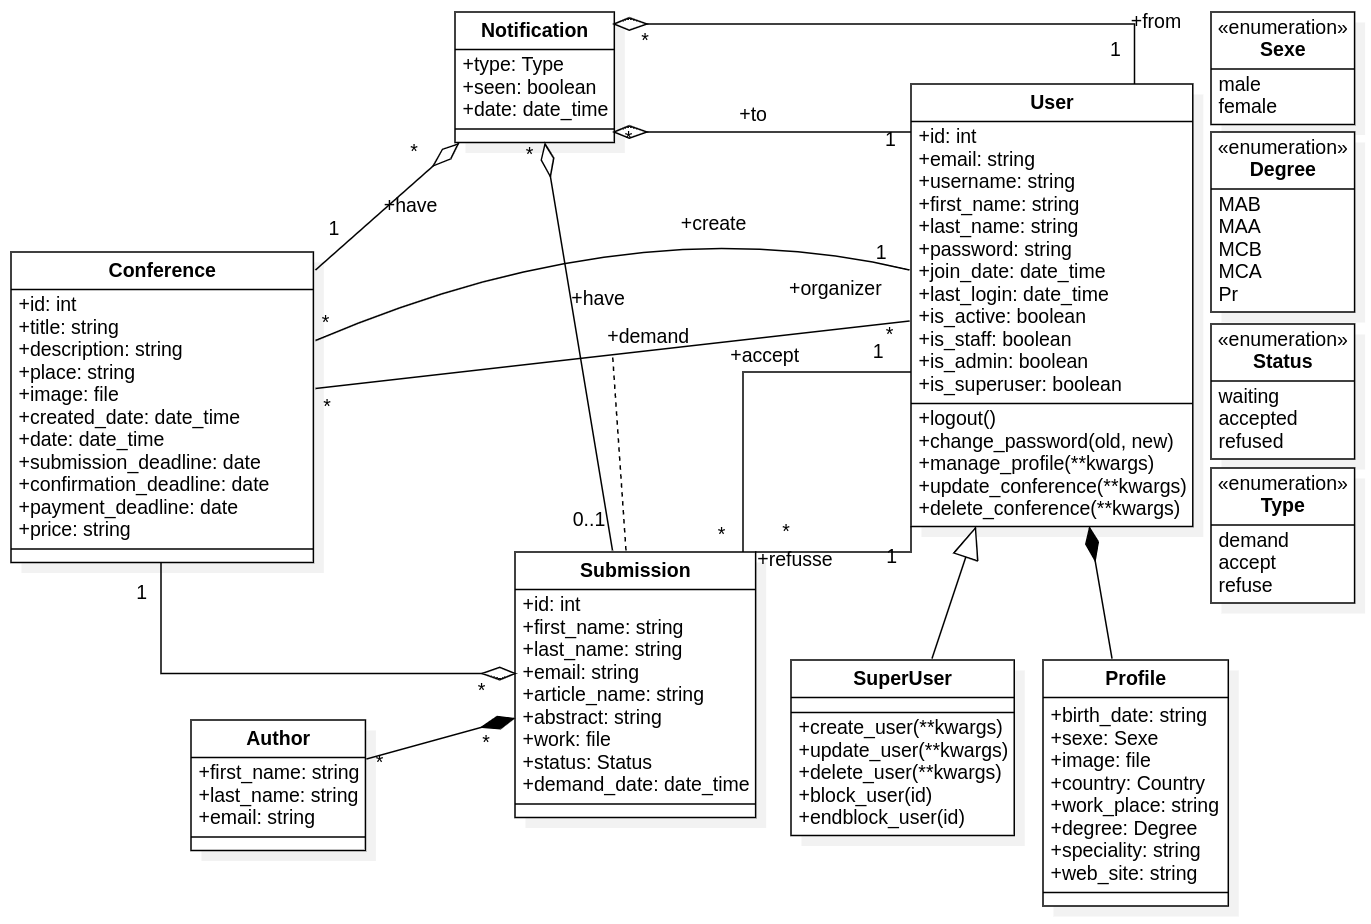
\includegraphics[width=\textwidth]{diagrams/class.png}
			\caption{class diagram}
			\label{fig:class-d}
		\end{figure}
	
	\subsection{Use case Diagram}
	\paragraph{}
	In Figure \ref{fig:use-case-d} we diagram to introduce what can every actor do in this project.
	\paragraph{}
	There is a guest who can register or login, and a user who can create, update, delete conferences and submission, or accept, confirm, refuse others submissions, and he can manage his profile (update country, degree, specialty... etc).
	\paragraph{}
	The superuser is who can do everything the user can do additionally to manage the database of the site.
	
		\begin{figure}[!ht]
			\centering
			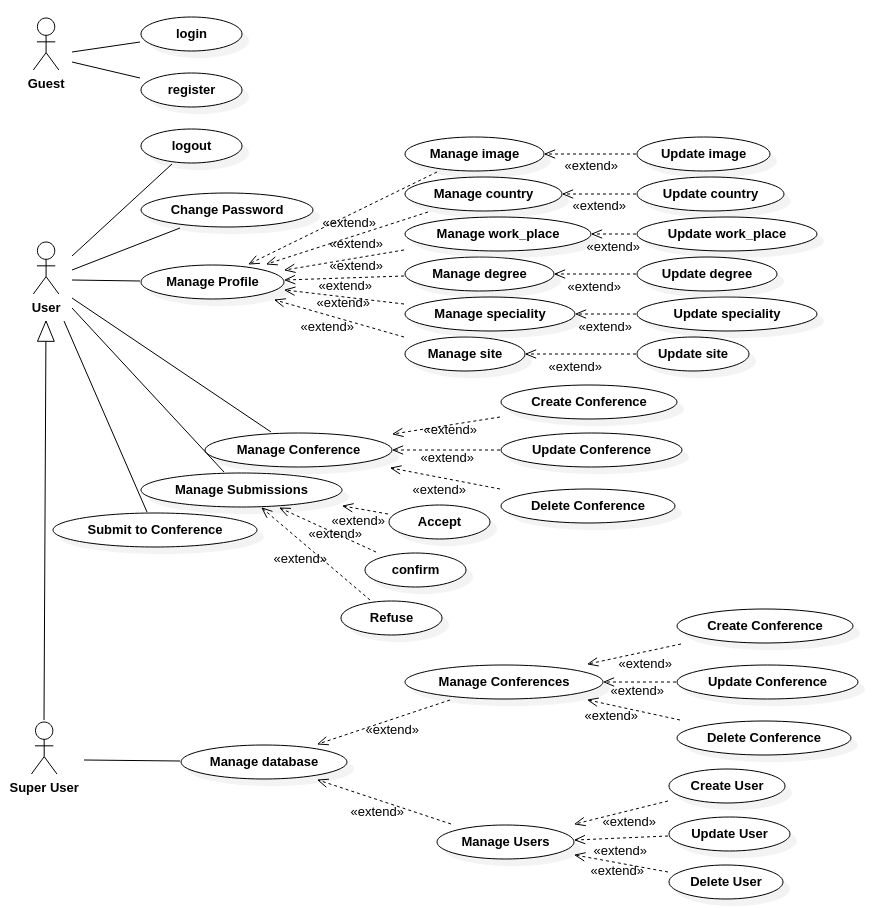
\includegraphics[width=\textwidth]{diagrams/use_case.png}
			\caption{use case diagram}
			\label{fig:use-case-d}
		\end{figure}
	
	\subsection{Sequence Diagrams}
	\paragraph{}
	Diagrams to figure out how each process is working behind the scene.
	\paragraph{}
	Because we have MVC design pattern in Django, all the sequence diagrams will contain a view, controller and a model for the process, when the view is the template of HTML that the user see, the controller is the back-end code to control the view and the model (the connection with the database).
	
	
	\subsubsection{For login}
	\paragraph{}
	In Figure \ref{fig:login-s-d} we have how the user can login.
	\paragraph{}
	The controller validate the data, in case of valid data he will redirected to profile page, or see errors.
	
		\begin{figure}[!ht]
			\centering
			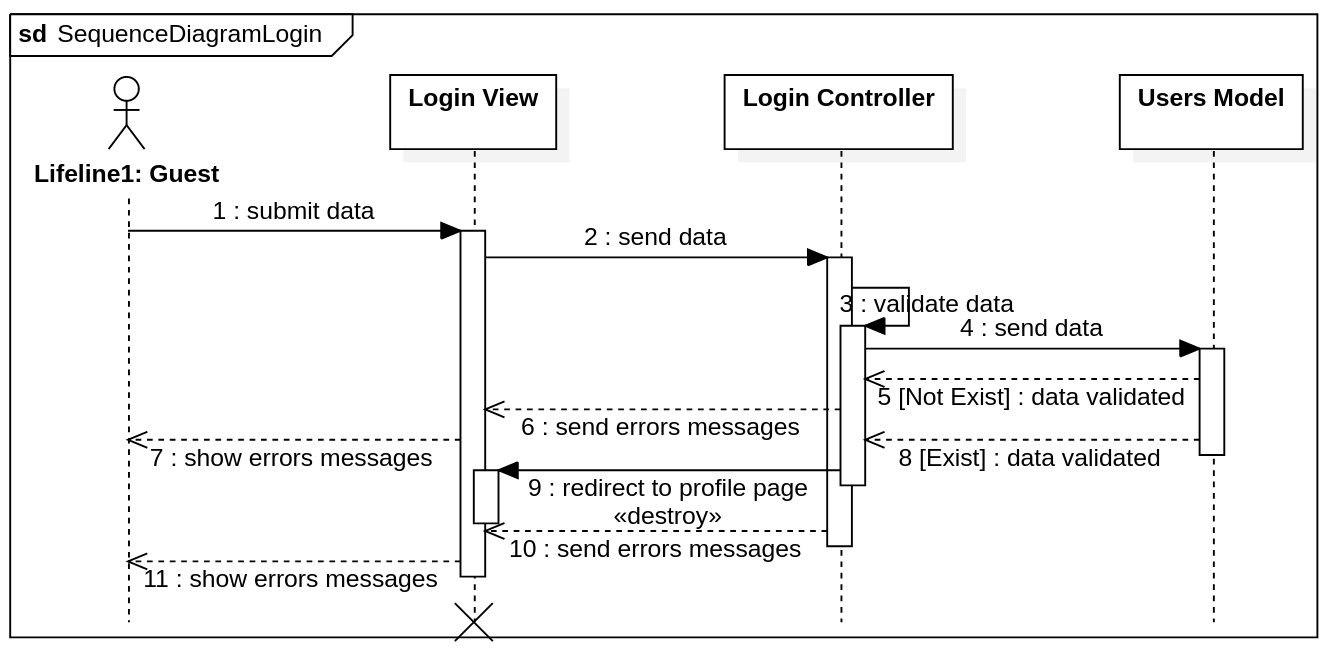
\includegraphics[width=\textwidth]{diagrams/login_sequence.png}
			\caption{login sequence diagram}
			\label{fig:login-s-d}
		\end{figure}
	
	\subsubsection{For register}
	\paragraph{}
	In Figure \ref{fig:register-s-d} we have how to register as a new user.
	\paragraph{}
	The controller validate the data and verify if exist in database, if valid he will create new user and redirect him to profile page, if not the user will see errors messages.
	
		\begin{figure}[!ht]
			\centering
			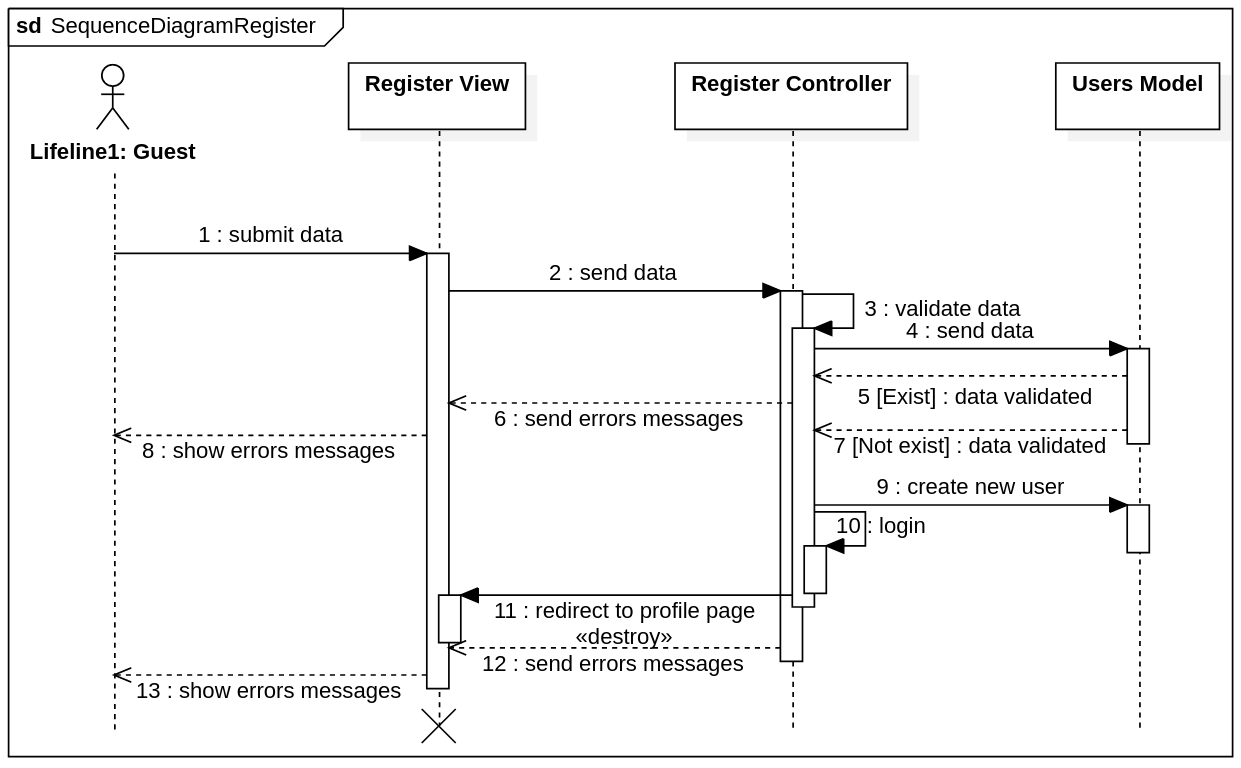
\includegraphics[width=\textwidth]{diagrams/register_sequence.png}
			\caption{register sequence diagram}
			\label{fig:register-s-d}
		\end{figure}
	
	\subsubsection{For create user}
	\paragraph{}
	In Figure \ref{fig:user-create-s-d} we have how to create new user.
	\paragraph{}
	The controller validate the data and verify the database(users model), in case of valid data he will create a new user successfully, or return errors messages to the view.
	
		\begin{figure}[!ht]
			\centering
			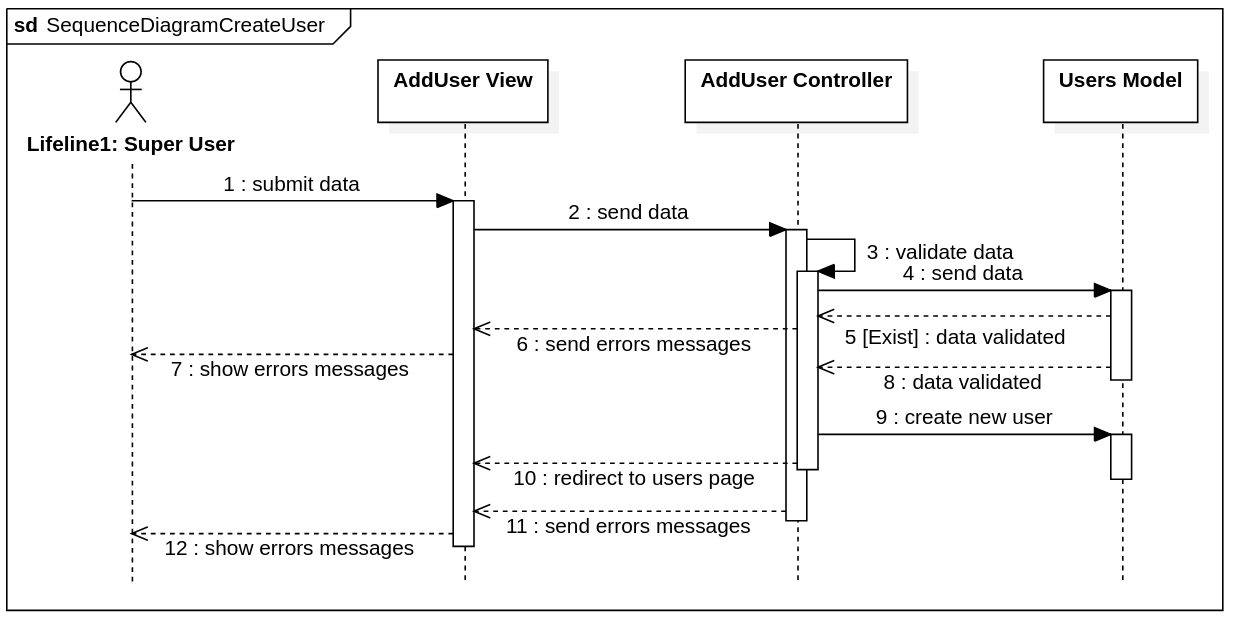
\includegraphics[width=\textwidth]{diagrams/user_create_sequence.png}
			\caption{create user sequence diagram}
			\label{fig:user-create-s-d}
		\end{figure}
	
	\subsubsection{For update user}
	\paragraph{}
	In Figure \ref{fig:user-update-s-d} we have how to update user information.
	\paragraph{}
	The controller validate the data and update the user in case of valid data, or return errors messages to the view.
	
		\begin{figure}[!ht]
			\centering
			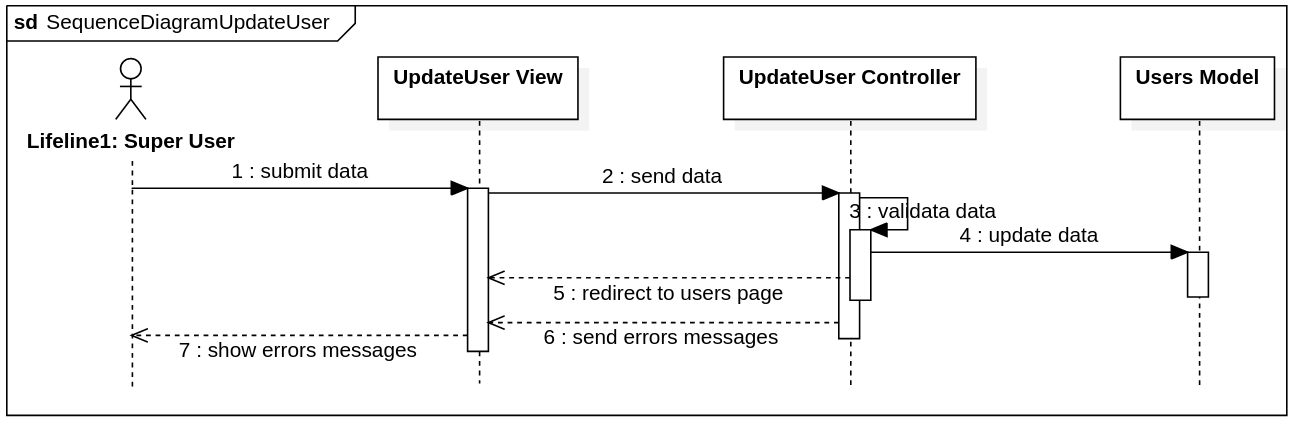
\includegraphics[width=\textwidth]{diagrams/user_update_sequence.png}
			\caption{update user sequence diagram}
			\label{fig:user-update-s-d}
		\end{figure}
	
	\subsubsection{For delete user}
	\paragraph{}
	In Figure \ref{fig:user-delete-s-d} we have how to delete a user from the data base.
	\paragraph{}
	The controller delete the user directly from the database and refresh the page.

		\begin{figure}[!ht]
			\centering
			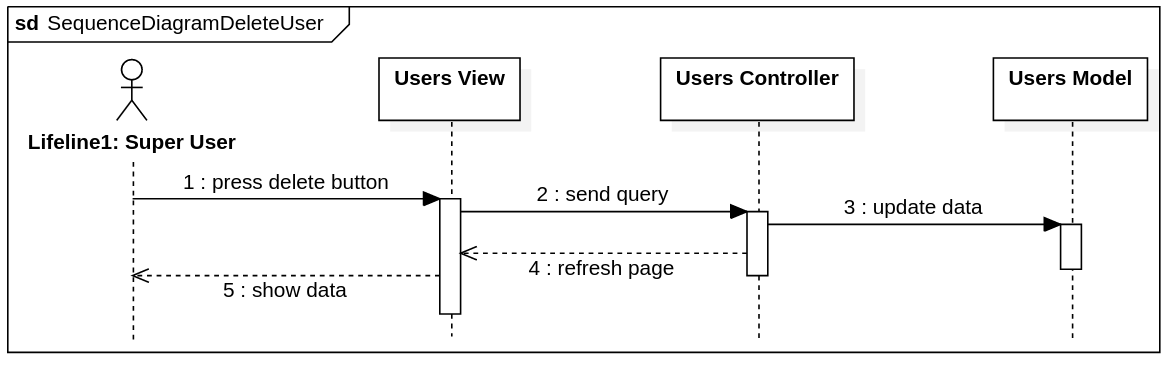
\includegraphics[width=\textwidth]{diagrams/user_delete_sequence.png}
			\caption{delete sequence diagram}
			\label{fig:user-delete-s-d}
		\end{figure}
	
	\subsubsection{For create conference}
	\paragraph{}
	In Figure \ref{fig:conference-create-s-d} we have how to create new user.
	\paragraph{}
	The controller validate the data of the conference that sent from the user to the view, and verify the database for duplicated data, then he will create new conference (with INSERT query in SQL Language) and redirect the user to the previous page or return errors messages to him.
	
		\begin{figure}[!ht]
			\centering
			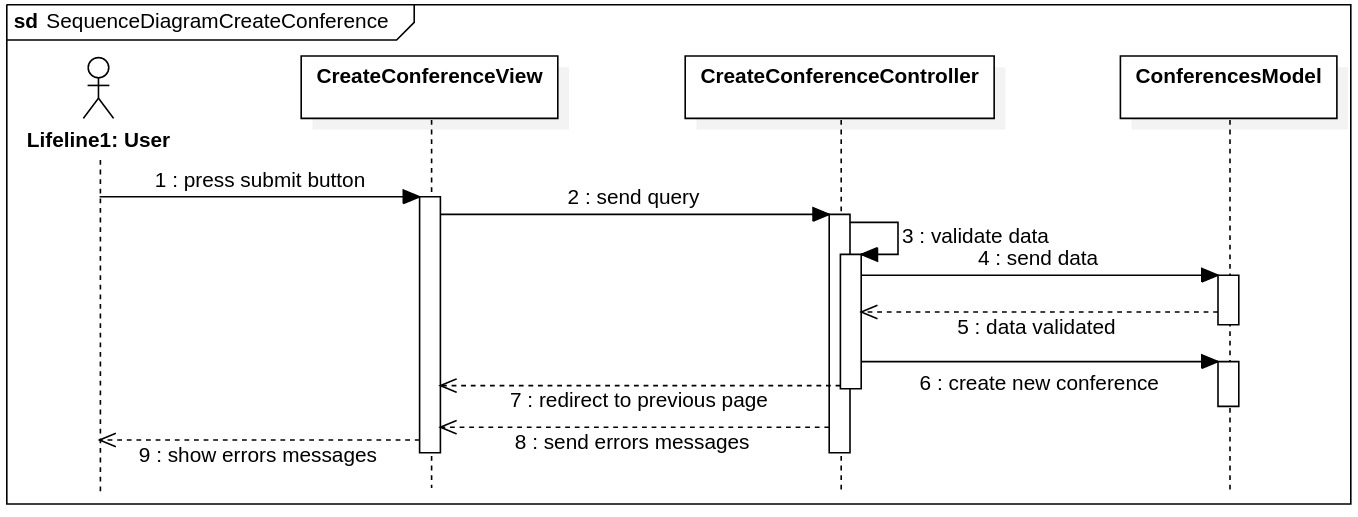
\includegraphics[width=\textwidth]{diagrams/conference_create_sequence.png}
			\caption{create user sequence diagram}
			\label{fig:conference-create-s-d}
		\end{figure}
	
	\subsubsection{For update conference}
	\paragraph{}
	In Figure \ref{fig:conference-update-s-d} we have how to update user information.
	\paragraph{}
	The controller validate the data of the conference that sent from the user to the view, and verify the database for duplicated data, then he will update this conference with the new data (with ALTER TABLE query in SQL Language) and redirect the user to the previous page or return errors messages to him.
	
		\begin{figure}[!ht]
			\centering
			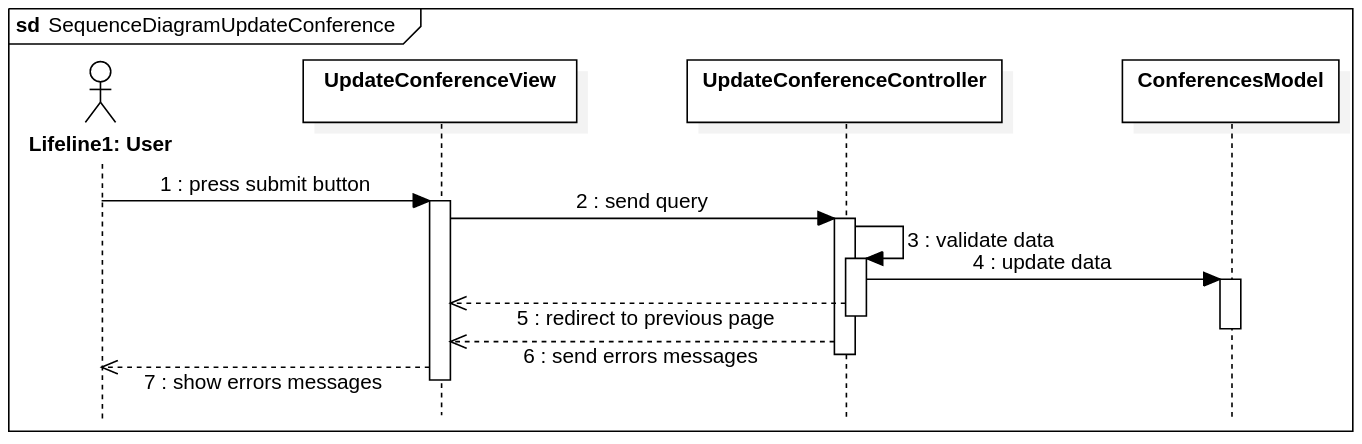
\includegraphics[width=\textwidth]{diagrams/conference_update_sequence.png}
			\caption{update user sequence diagram}
			\label{fig:conference-update-s-d}
		\end{figure}
	
	\subsubsection{For delete conference}
	\paragraph{}
	In Figure \ref{fig:conference-delete-s-d} we have how to delete a user from the data base.
	\paragraph{}
	Same as user delete process.
	
		\begin{figure}[!ht]
			\centering
			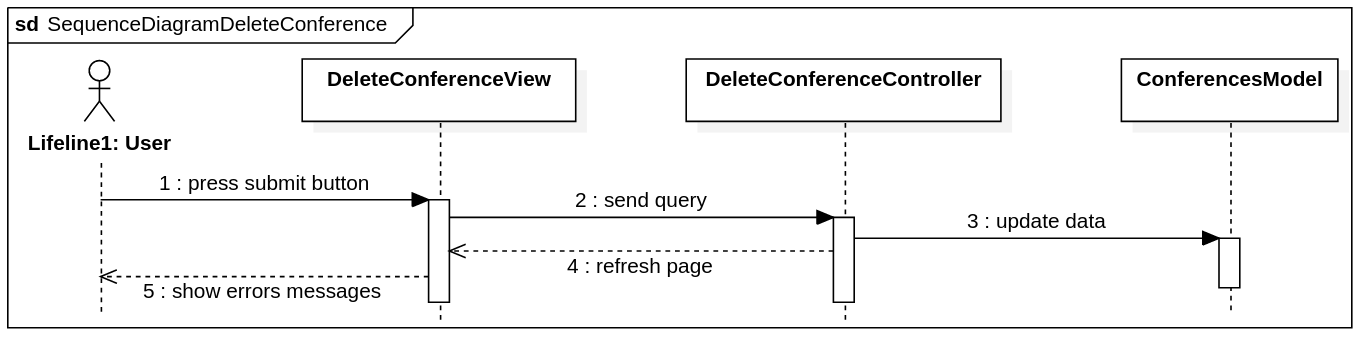
\includegraphics[width=\textwidth]{diagrams/conference_delete_sequence.png}
			\caption{delete sequence diagram}
			\label{fig:conference-delete-s-d}
		\end{figure}
	
	\subsubsection{For create submission}
	\paragraph{}
	In Figure \ref{fig:submission-create-s-d} we have how to create new user.
	
		\begin{figure}[!ht]
			\centering
			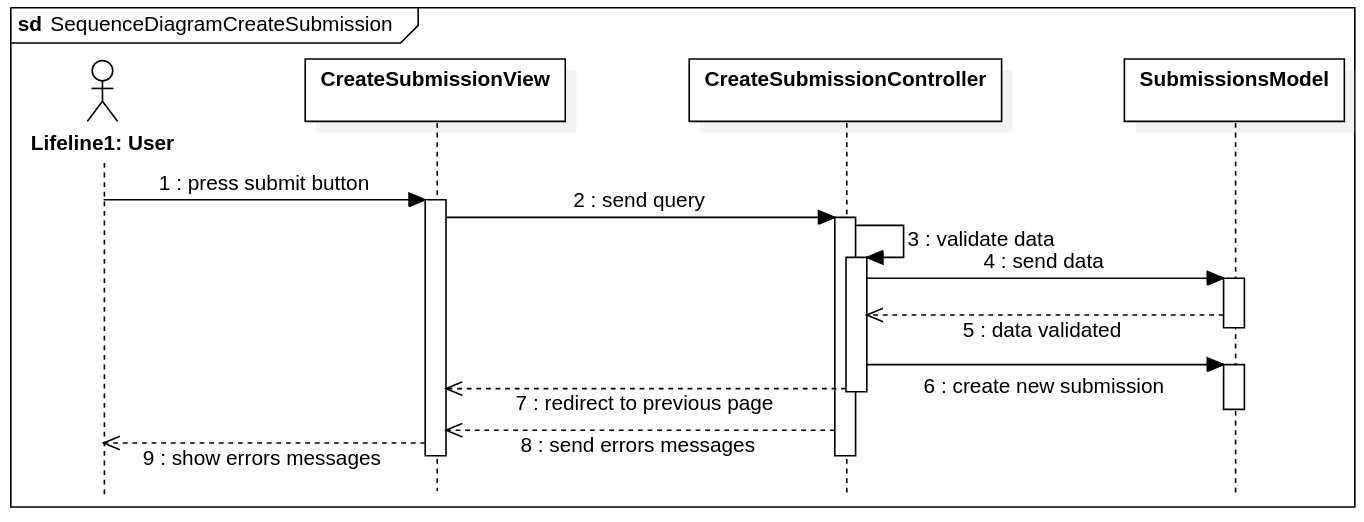
\includegraphics[width=\textwidth]{diagrams/submission_create_sequence.png}
			\caption{create user sequence diagram}
			\label{fig:submission-create-s-d}
		\end{figure}
	
	\subsubsection{For update submission}
	\paragraph{}
	In Figure \ref{fig:submission-update-s-d} we have how to update user information.
	
		\begin{figure}[!ht]
			\centering
			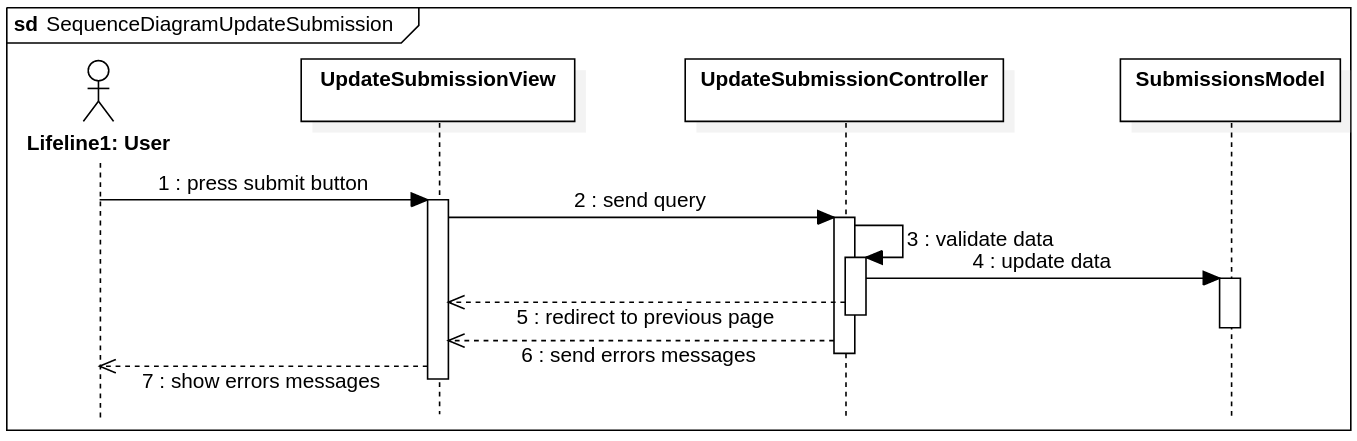
\includegraphics[width=\textwidth]{diagrams/submission_update_sequence.png}
			\caption{update user sequence diagram}
			\label{fig:submission-update-s-d}
		\end{figure}
	
	\subsubsection{For delete submission}
	\paragraph{}
	In Figure \ref{fig:submission-delete-s-d} we have how to delete a user from the data base.
	
		\begin{figure}[!ht]
			\centering
			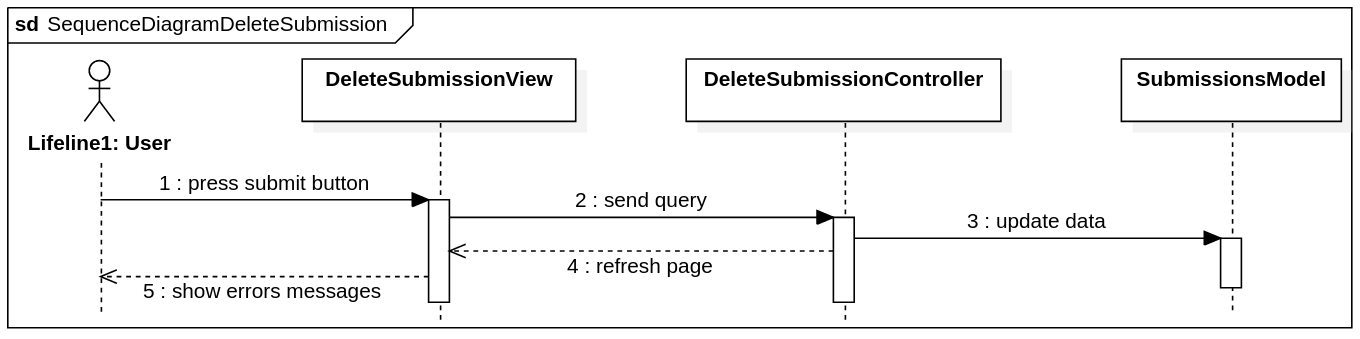
\includegraphics[width=\textwidth]{diagrams/submission_delete_sequence.png}
			\caption{delete sequence diagram}
			\label{fig:submission-delete-s-d}
		\end{figure}